% Figure s02f04_dirac (Session 2): the honeycomb lattice, the phasor sum and the two cones.
% The image is rendered by figures/blender/s02f04_dirac.py; the coordinates of the labels come from
% figures/blender/out/s02f04_dirac_anchors.tex. Build with figures/blender/build_figure.sh s02f04_dirac.
\documentclass[11pt,tikz,border=0pt]{standalone}
\usepackage[T1]{fontenc}
\usepackage{amsmath,amssymb,graphicx,bm}
\usepackage{xcolor}
\usetikzlibrary{arrows.meta,calc}
% The three label colors of the figures, with the same values as in src/figures_preamble.tex.
\definecolor{aqmaccent}{RGB}{31,78,121}
\definecolor{aqmbroken}{RGB}{168,42,34}
\definecolor{aqmmuted}{RGB}{125,125,125}

\newlength{\figw}\setlength{\figw}{15.6cm}   % the text width of the notes (A4, 2.7 cm margins)

\begin{document}
\begin{tikzpicture}[lbl/.style={font=\small, inner sep=1.5pt}, pnl/.style={font=\small\bfseries, inner sep=1.5pt}]
  \node[anchor=south west, inner sep=0pt] at (0,0)
    {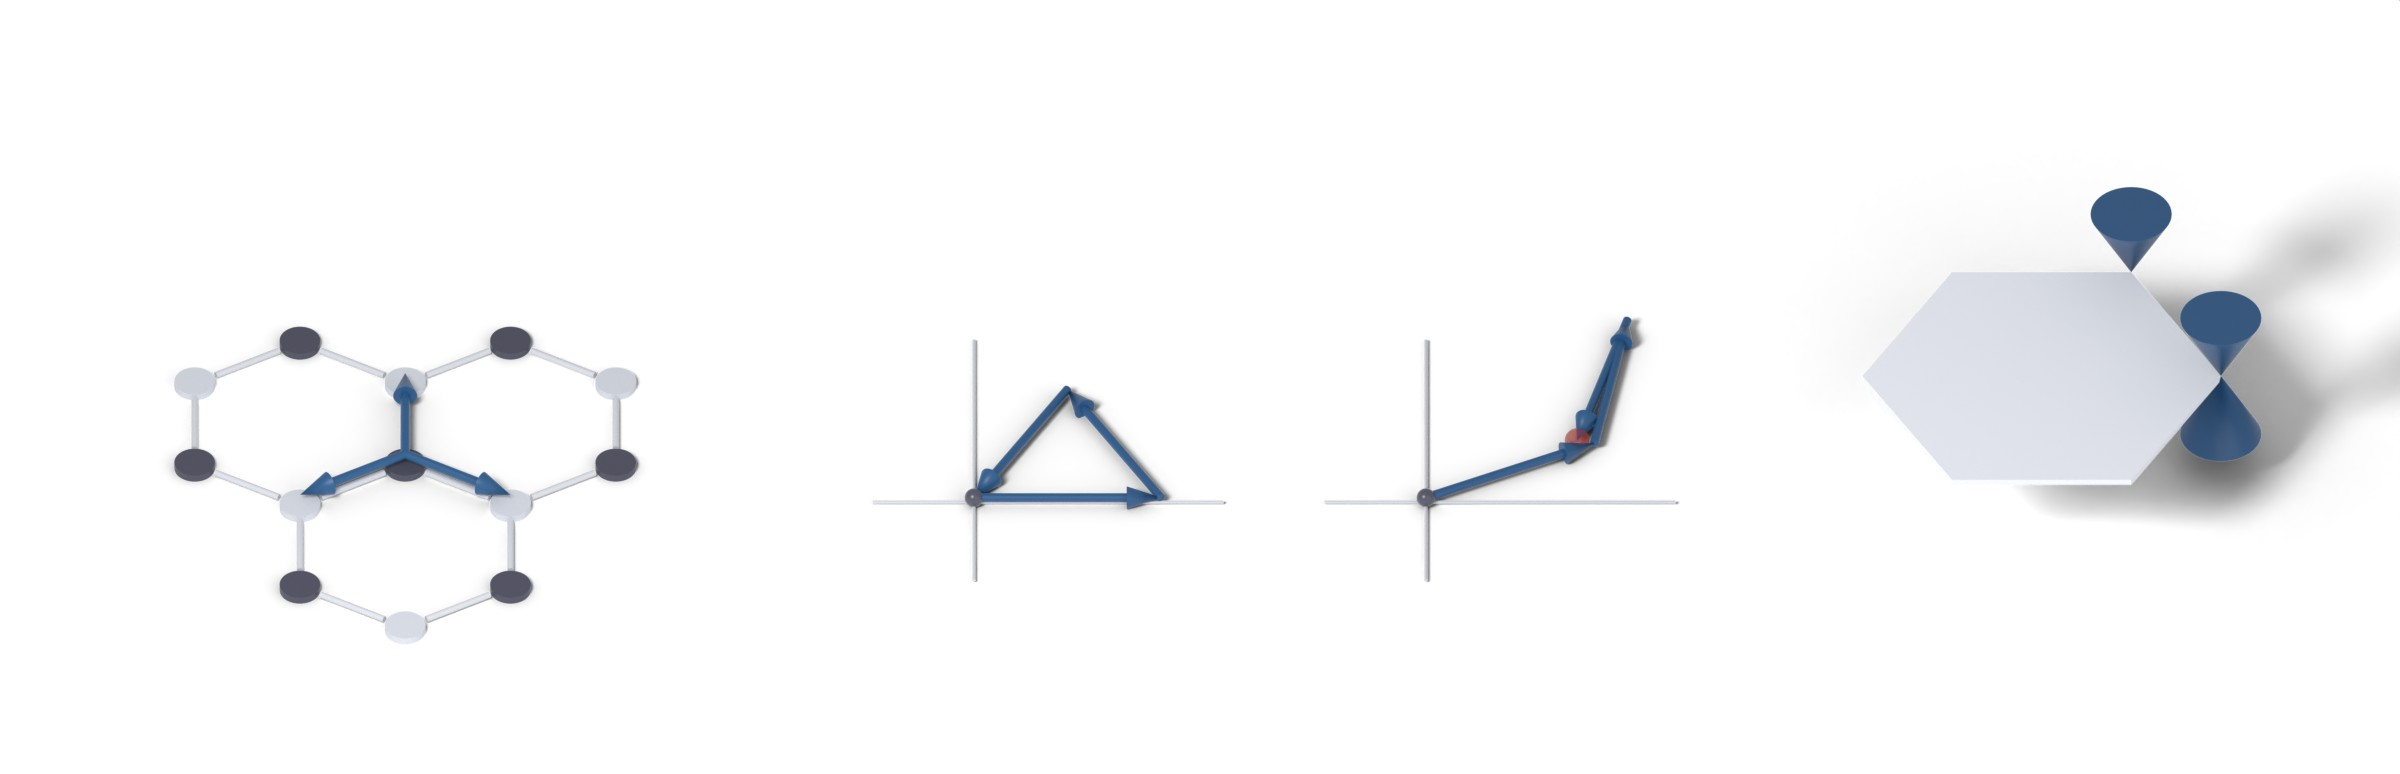
\includegraphics[width=\figw]{../blender/out/s02f04_dirac.jpg}};
  %% written by figlib.py; x and y in units of the image width
\coordinate (ad1) at (0.1688\figw,0.1756\figw);
\coordinate (ad2) at (0.2237\figw,0.1121\figw);
\coordinate (ad3) at (0.1140\figw,0.1121\figw);
\coordinate (aA) at (0.1571\figw,0.1271\figw);
\coordinate (apanel) at (0.0325\figw,0.2144\figw);
\coordinate (bK) at (0.4286\figw,0.0645\figw);
\coordinate (bk) at (0.6169\figw,0.0645\figw);
\coordinate (bpanel) at (0.3506\figw,0.2144\figw);
\coordinate (cK) at (0.9383\figw,0.1958\figw);
\coordinate (cKp) at (0.8945\figw,0.2466\figw);
\coordinate (cGamma) at (0.8506\figw,0.1668\figw);
\coordinate (cpanel) at (0.7273\figw,0.2144\figw);

  \node[pnl, anchor=west] at (apanel) {(a)};
  \node[pnl, anchor=west] at (bpanel) {(b)};
  \node[pnl, anchor=west] at (cpanel) {(c)};
  \node[lbl, text=aqmaccent] at (ad1) {$\bm\delta_1$};
  \node[lbl, text=aqmaccent] at (ad2) {$\bm\delta_2$};
  \node[lbl, text=aqmaccent] at (ad3) {$\bm\delta_3$};
  \node[lbl, anchor=north east] at (aA) {$A$};
  \node[lbl, anchor=north] at (bK) {at $\mathbf K$, closed};
  \node[lbl, anchor=north] at (bk) {generic $\mathbf k$, open};
  \node[lbl, anchor=south west] at (cK) {$K$};
  \node[lbl, anchor=south west] at (cKp) {$K'$};
  \node[lbl, anchor=south, text=aqmmuted] at (cGamma) {$\Gamma$};
\end{tikzpicture}
\end{document}
